\chapter{Technical Implementation}
\label{ch:implementation}

This chapter details the technical architecture and implementation of the TCM-Sage system. The implementation focuses on three core pillars: a retrieval-augmented generation (RAG) pipeline optimized for classical Traditional Chinese Medicine (TCM) texts, a knowledge graph (KG) integration for structured entity resolution, and a blind A/B evaluation framework (Arena) for performance benchmarking.

\section{Technology Stack}

The system is built on a full-stack architecture with the following components:

\subsection{Backend Infrastructure}
The backend is implemented using \textbf{Python 3.13}, utilizing the \textbf{FastAPI} framework for high-concurrency asynchronous API handling. The core orchestration layer uses \textbf{LangChain}, which provides the abstraction for retrieval chains and prompt templates. Data persistence for vectorized text is managed by \textbf{ChromaDB}, an open-source vector database chosen for its local persistence capabilities and efficient metadata filtering.

\subsection{Frontend and User Interface}
The user interface is developed with \textbf{Next.js 16} (App Router) and \textbf{React 19}. \textbf{TypeScript} ensures type safety across the application, while \textbf{Tailwind CSS} is used for responsive, utility-first styling. The interface supports a dual-stream architecture for the Arena evaluation system, allowing simultaneous rendering of two independent Large Language Model (LLM) responses.

\subsection{Language Models and Embeddings}
\begin{itemize}
    \item \textbf{LLM:} The system utilizes the \textbf{DashScope API} (Qwen series), specifically targeting the international endpoint (\texttt{dashscope-intl.aliyuncs.com}) for consistent availability.
    \item \textbf{Embedding Model:} \textbf{DashScope text-embedding-v4} (1024 dimensions) with TCM domain-specific asymmetric prefixes. Ingestion uses the prefix ``Generate semantic representation for this classical TCM text for retrieval'' while queries use ``Generate semantic representation for this TCM clinical question to retrieve relevant classical passages.'' This asymmetric strategy follows DashScope best practices for domain-specific retrieval.
    \item \textbf{Reranker:} \textbf{qwen3-rerank} cross-encoder, wired into the \texttt{hybrid\_search()} pipeline. The reranker operates on vector search results \textit{before} combining with knowledge graph results, as KG facts (structured entity relationships) do not benefit from semantic reranking. Both the original distance score and the reranker's relevance score are preserved in metadata for downstream use.
\end{itemize}

\subsection{Knowledge Graph and Local Support}
The structural backbone for entity resolution is \textbf{SymMap v2.0}, implemented using the \textbf{NetworkX} library. A custom \textit{crosswalk bridge} was developed to map colloquial and modern medical terms to classical TCM entities. For researchers requiring local privacy, the system supports local LLM deployment via \textbf{Ollama} and \textbf{LMStudio} through standard OpenAI-compatible endpoints.

\section{Data Acquisition and Preprocessing}

The quality of a RAG system is fundamentally bounded by its underlying corpus. TCM-Sage utilizes a curated set of 17 classical TCM texts, totaling 3.72 million characters in UTF-8 encoding.

\subsection{Chunking Strategies}
To preserve the semantic integrity of classical texts, two distinct chunking strategies were implemented:
\begin{enumerate}
    \item \textbf{Chapter-based Chunking:} Applied to the majority of the corpus, where texts are split by \textit{Pianming} (chapter title) markers. This results in an average chunk size of approximately 500 characters, providing sufficient context for general theoretical queries.
    \item \textbf{Clause-level Chunking:} Specifically for \textit{Shanghan Lun} (388 clauses) and \textit{Jingui Yaolue} (489 clauses). Using regex pattern matching on numerical markers (e.g., "N."), the system extracts individual clinical clauses. This granularity is essential for formula-based retrieval where specific symptom-sign clusters are defined within a single clause.
\end{enumerate}

\subsection{Contextual Header Prepend}
To improve embedding quality and retrieval precision, each chunk is prepended with a \textit{Contextual Header}. For example, a clause from \textit{Shanghan Lun} is transformed into: \texttt{"<Shanghan Lun> Clause 35 Mahuang Tang: [Clause Content]"}. This ensures that even if the clause text itself is brief, the vector representation captures the source book and the associated formula name.

\subsection{Ingestion and Storage}
The ingestion pipeline handles the DashScope batch limit of 10 embeddings per API call through a robust checkpoint/resume system. This prevents data loss during network interruptions or API rate limiting. The final processed corpus consists of 12,204 chunks, requiring approximately 850MB of \textbf{ChromaDB} persistent storage.

\section{Retrieval Pipeline Implementation}

The retrieval pipeline is engineered to address the specific nuances of classical TCM literature, where source authority and formula-specific contexts are paramount.

\subsection{Formula-Aware Canonical Retrieval}
Standard vector search often fails to prioritize the \textit{source} text of a formula. We implemented a specialized detection layer:
\begin{enumerate}
    \item Detect formula names (e.g., \textit{Guizhi Tang}) in the user query.
    \item Perform a metadata-filtered ChromaDB search restricted to canonical texts (\textit{Shanghan Lun} and \textit{Jingui Yaolue}).
    \item Prepend these canonical results to the general retrieval list, ensuring the "original" definition is always present in the context.
\end{enumerate}

\subsection{Multi-Clause Comparison}
TCM practitioners frequently compare different clauses to differentiate syndromes. The system implements an \texttt{extract\_clause\_references} function using \texttt{re.finditer}. It supports various citation formats (with or without "Section" or "Clause" markers) and can retrieve multiple non-contiguous clauses in a single query.

\subsection{Source Authority Boost}
A \textit{Source Chronological Boost} (\texttt{\_SOURCE\_CHRONOLOGICAL\_BOOST}) dictionary applies multipliers (ranging from 0.90 to 0.97) to the distance scores of older, more authoritative texts. This mathematically "pulls" foundational Han Dynasty texts closer to the query than later, more verbose Ming or Qing Dynasty commentaries.

\subsection{Deduplication and Filtering}
To maximize the diversity of information within the context window:
\begin{itemize}
    \item \textbf{Broader Retrieval:} The system initially retrieves $k \times 3$ results before truncation.
    \item \textbf{Source Deduplication:} Only the most relevant chunk per \textit{book + chapter} combination is retained, preventing the LLM from being overwhelmed by repetitive content from a single source.
    \item \textbf{ChromaDB Filters:} Complex filtering uses the \texttt{\$and} operator (e.g., \texttt{'\$and': [\{'clause\_number': num\}, \{'book': name\}]}), as flat dictionaries are ignored by the ChromaDB filter parser.
\end{itemize}

\section{Knowledge Graph Integration}

The SymMap v2.0 knowledge graph provides a structured layer of medical knowledge that complements the unstructured text retrieval.

\subsection{Graph Architecture}
The graph contains 18,450 entities and 21,476 relationships. Key entity types include \textit{Herbs}, \textit{Symptoms}, \textit{TCM Syndromes} (Zheng), and \textit{Modern Diseases}.

\subsection{Entity Matching and Crosswalk}
Mapping modern user queries to classical graph entities is achieved through:
\begin{itemize}
    \item \textbf{Jieba Segmentation:} Tokenizing the query into candidate medical terms.
    \item \textbf{Alias Mapping:} A crosswalk bridge that translates colloquial modern Chinese terms to formal TCM terminology (e.g., ``du zi teng'' [belly ache] $\rightarrow$ ``fu tong'' [abdominal pain], ``shui bu zhao'' [can't sleep] $\rightarrow$ ``shi mian'' [insomnia]).
    \item \textbf{BFS Traversal:} Upon matching an entity, the system performs a Breadth-First Search (BFS) with configurable depth (default 2) to retrieve related symptoms or herbs, providing the LLM with structured diagnostic relationships.
\end{itemize}

\section{Generation and Prompt Engineering}

The generation layer is optimized to ensure the LLM adheres to professional TCM methodologies while maintaining strict formatting. The system supports eight LLM providers through a unified \texttt{create\_llm()} factory function, enabling seamless switching between cloud APIs (DashScope, OpenAI, Anthropic, Google, OpenRouter, Together) and local inference (Ollama, LMStudio).

\subsection{Query Classification}
Each incoming query is first classified by a dedicated classifier LLM (temperature 0.0) into \texttt{informational} or \texttt{prescriptive} categories using \texttt{get\_query\_severity()}. The classification determines which pre-initialized LLM instance handles the query:

\begin{itemize}
    \item \texttt{llm\_informational}: temperature 0.7 for general knowledge queries
    \item \texttt{llm\_prescriptive}: temperature 0.0 for clinical/formula queries
\end{itemize}

The classifier, main LLMs, and verifier can each be configured with independent providers and models via environment variables, allowing fine-grained control over cost and quality trade-offs.

\subsection{System Prompt Architecture}
We use \texttt{ChatPromptTemplate.from\_messages()} to maintain a clean separation between the \texttt{SystemMessage} and the \texttt{UserMessage}. Empirical testing showed that merging these into a single string caused the model to ignore complex formatting constraints.

The \texttt{DEFAULT\_SYSTEM\_PROMPT} incorporates several professional frameworks:
\begin{itemize}
    \item \textbf{Bian Zheng Lun Zhi:} Standard diagnostic and treatment framework.
    \item \textbf{Yuanliu Methodology:} Tracing the origin and evolution of formulas across different sources.
    \item \textbf{Jun Chen Zuo Shi:} Drug hierarchy analysis (Sovereign, Minister, Assistant, Courier).
    \item \textbf{Measurement Conversion:} A hard-coded Han Dynasty conversion table (1 \textit{liang} $\approx$ 13.8g), correcting the common LLM hallucination of 1 \textit{liang} $\approx$ 3g.
\end{itemize}

\subsection{Context Anchoring and Pattern Priming}
To prevent ``context drift,'' we use a boundary marker (\texttt{=== End of References ===}) followed by a \texttt{[Formatting Requirements]} section placed \textit{after} the retrieved context. This ``post-context anchoring'' ensures the most recent tokens the LLM sees are the instructions, not the data. Furthermore, we discovered \textit{Pattern Priming}: by formatting the RAG context as clean Markdown (using headers and blockquotes), the LLM naturally mirrors this structured output format without explicit instruction.

\section{Arena Evaluation System}

To provide an objective measure of RAG effectiveness, we implemented a blind A/B testing framework in \texttt{arena.py}.

\subsection{Baseline Configuration}
The ``Plain LLM'' baseline uses a generic ``helpful assistant'' prompt and has access to \textbf{DuckDuckGo Search} (\texttt{ddgs} package) to simulate a general-purpose AI's ability to retrieve information from the web. This represents a representative general-purpose configuration for non-specialized models.

\subsection{Asynchronous Dual Streaming}
The system uses \texttt{asyncio.Queue} and \texttt{asyncio.gather} to stream responses from both the TCM-Sage pipeline and the baseline simultaneously. A random position assignment (A/B) ensures voters cannot identify the system by its position on the screen.

\subsection{Reliability and Storage}
A 60-second timeout per stream prevents the UI from hanging if one backend fails. All interaction data, including the query, both responses, and the final vote, are stored in a \textbf{JSONL} format with timestamps for later statistical analysis.

\section{Web Application Implementation}

The frontend is designed to be a professional clinical tool, prioritizing clarity and traceability.

\subsection{Internationalization and State}
The system supports Traditional Chinese (default), Simplified Chinese, and English. Language state is managed via \textbf{React Context}, with translations loaded from static JSON files.

\subsection{UX Enhancements}
\begin{itemize}
    \item \textbf{Smart Auto-scroll:} The chat interface automatically scrolls with new content but "unlocks" if the user manually scrolls up to read previous messages, showing a floating "down" button for quick return.
    \item \textbf{Citation Panel:} Clicking a citation number opens a side panel displaying the full source text and a mini knowledge graph view (built with xyflow/React Flow) showing the entity and its immediate relationships.
    \item \textbf{KG Explorer:} A dedicated \texttt{/kg/[entityId]} route provides a full-page \textbf{Cytoscape.js} graph explorer, allowing users to browse the knowledge graph, expand nodes on click, and search for specific entities.
\end{itemize}

\begin{figure}[H]
\centering
\begin{minipage}{0.48\textwidth}
    \centering
    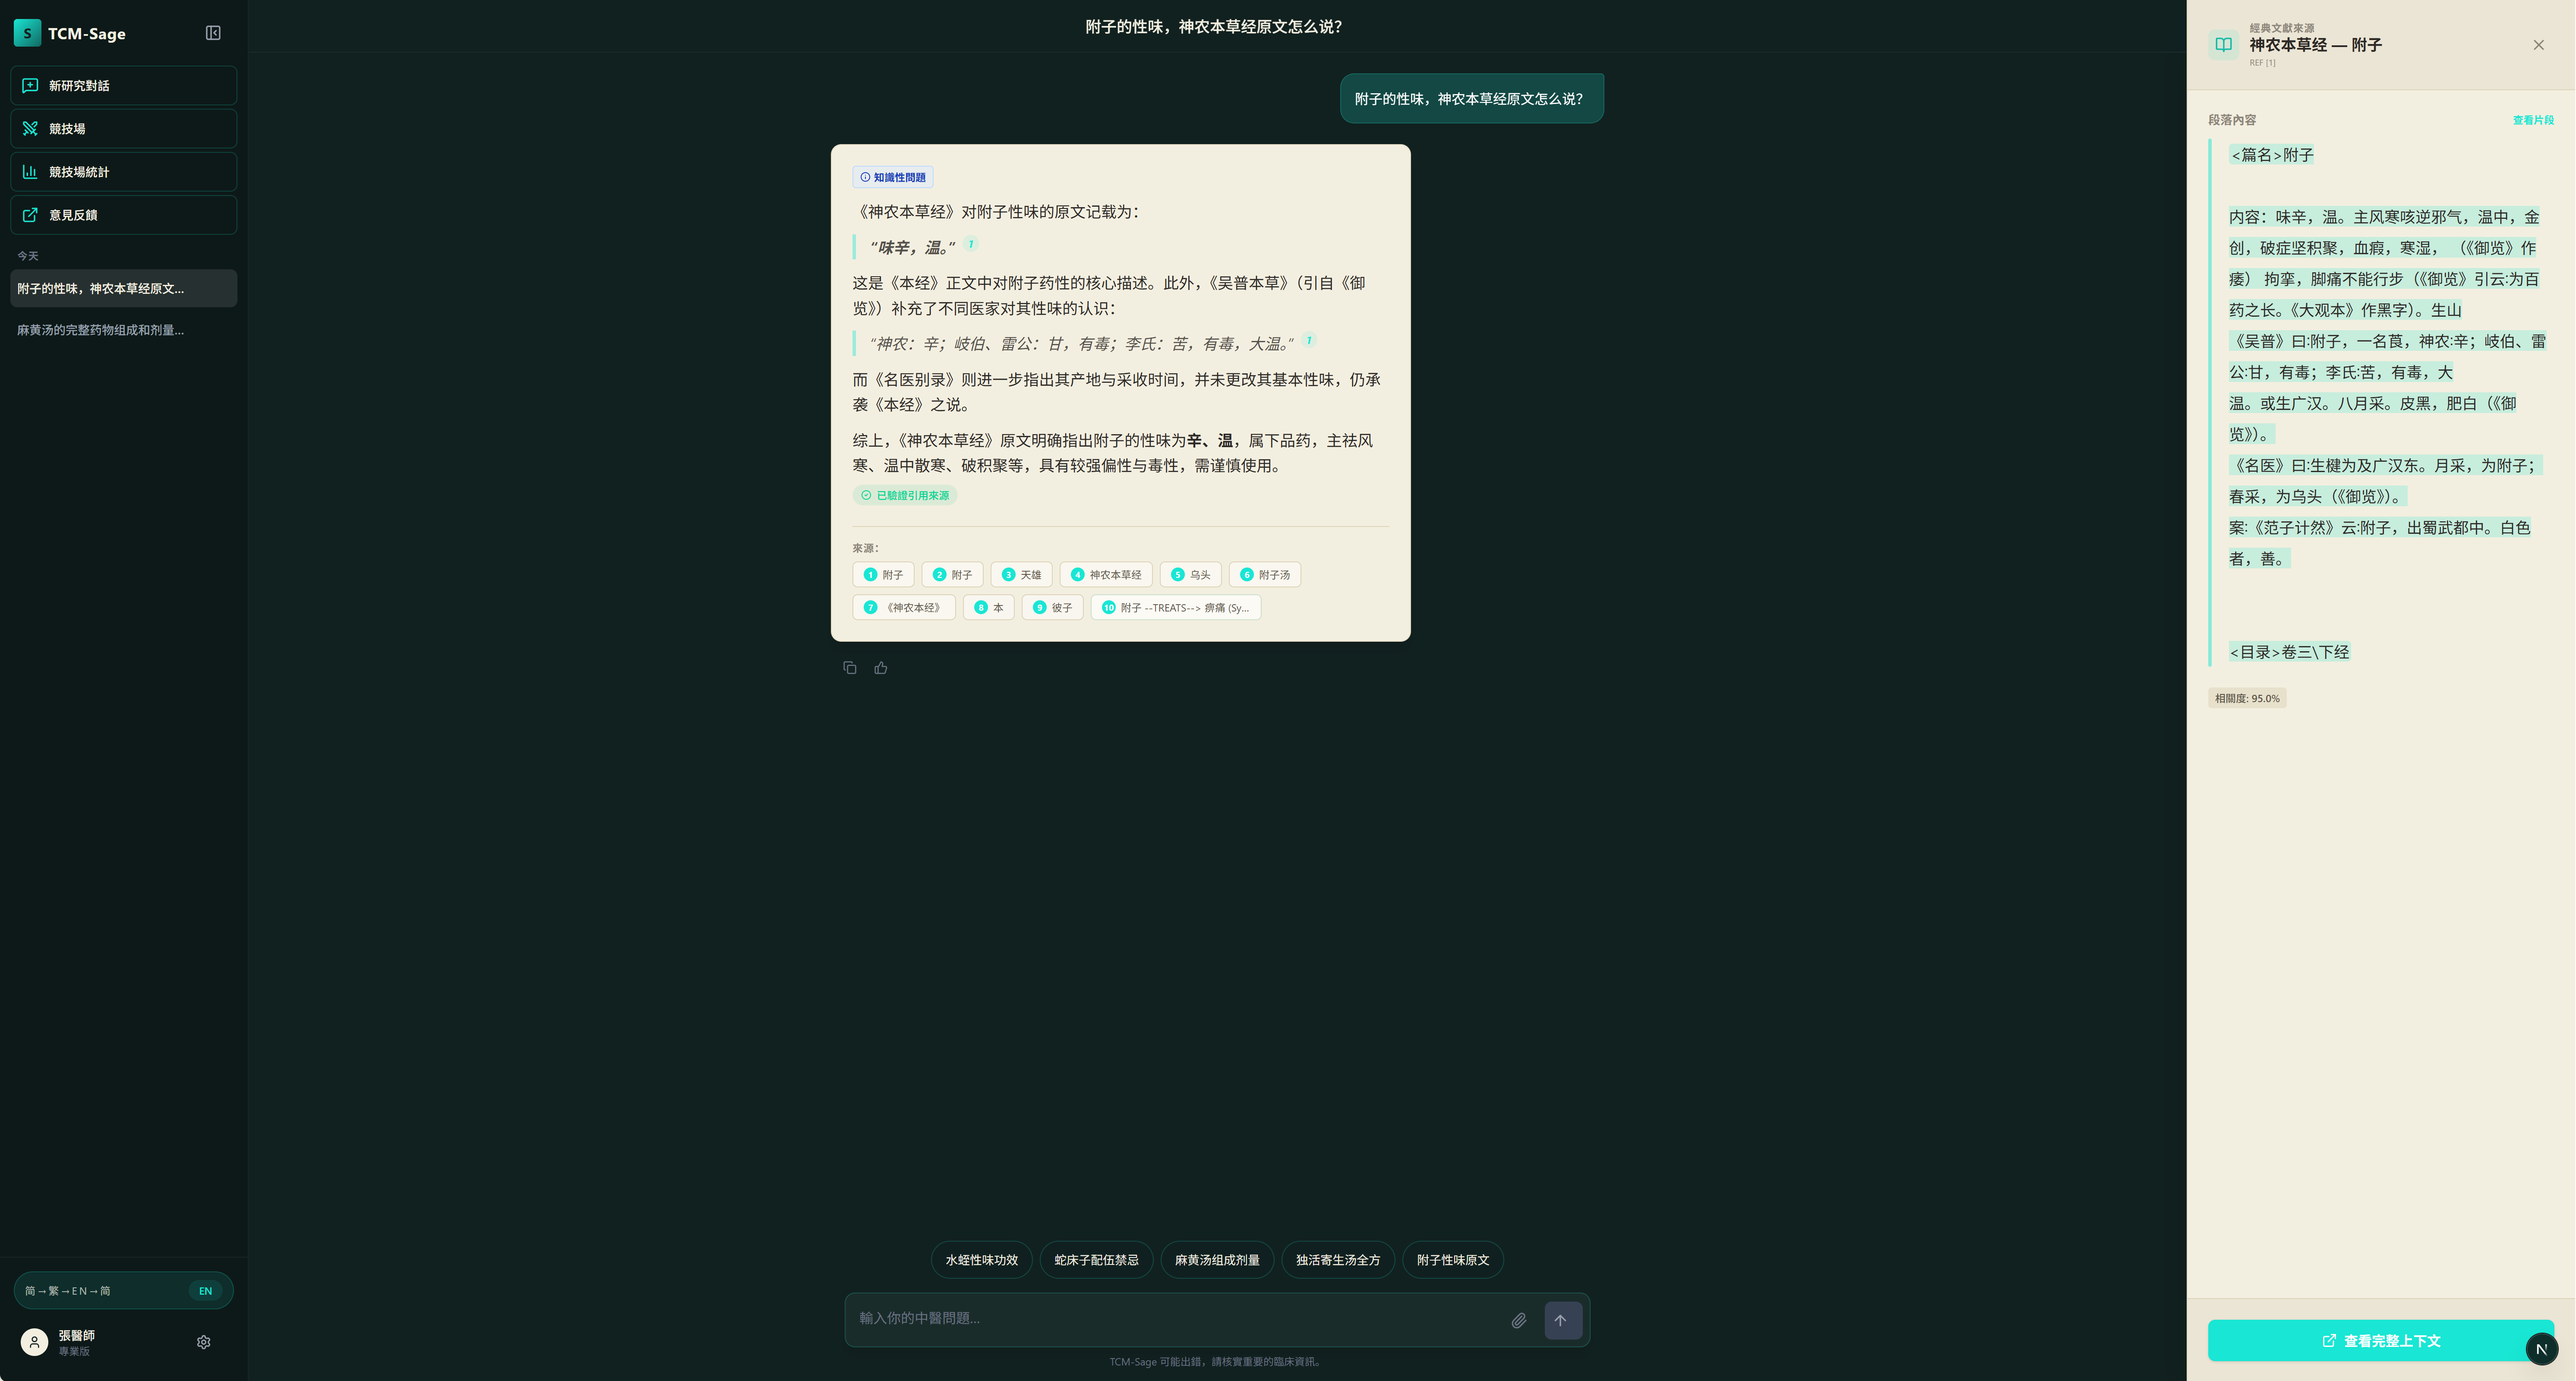
\includegraphics[width=\textwidth]{figures/ui-main-chat.png}
    \caption{Citation Panel showing the original source text with click-through to full passage.}
    \label{fig:ui_main}
\end{minipage}\hfill
\begin{minipage}{0.48\textwidth}
    \centering
    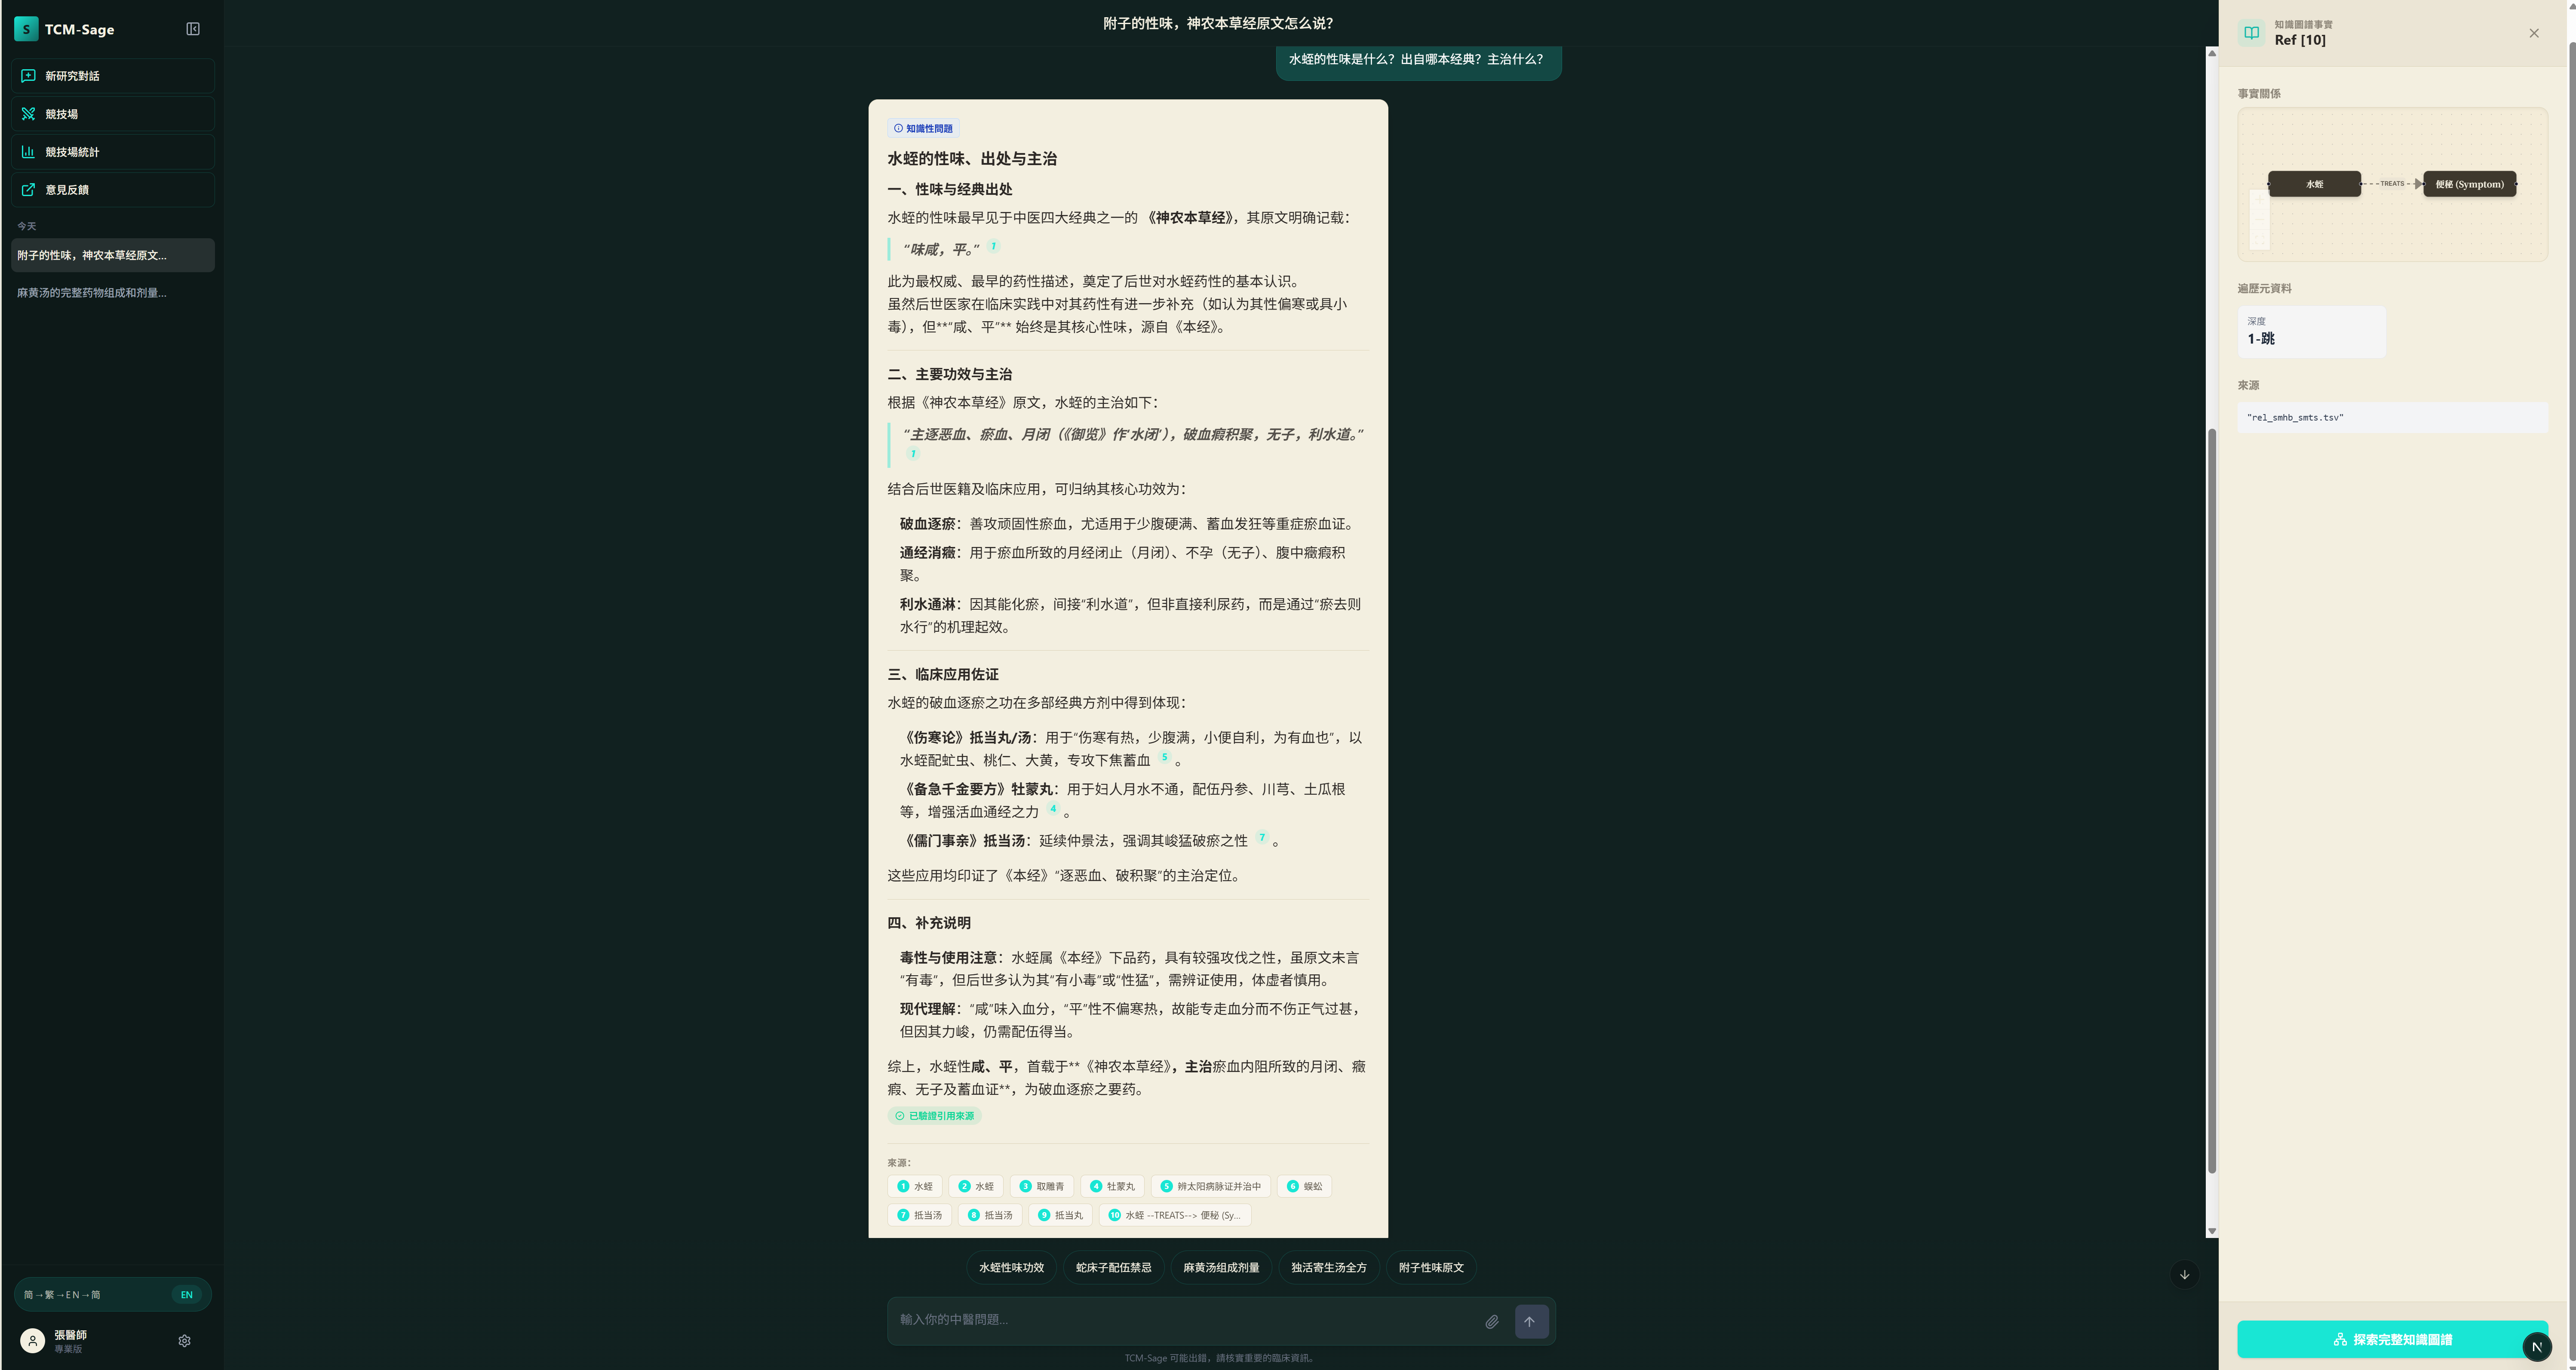
\includegraphics[width=\textwidth]{figures/ui-kg-main-chat.png}
    \caption{Citation Panel showing the mini knowledge graph view for an entity.}
    \label{fig:ui_kg_cite}
\end{minipage}
\end{figure}

\begin{figure}[H]
\centering
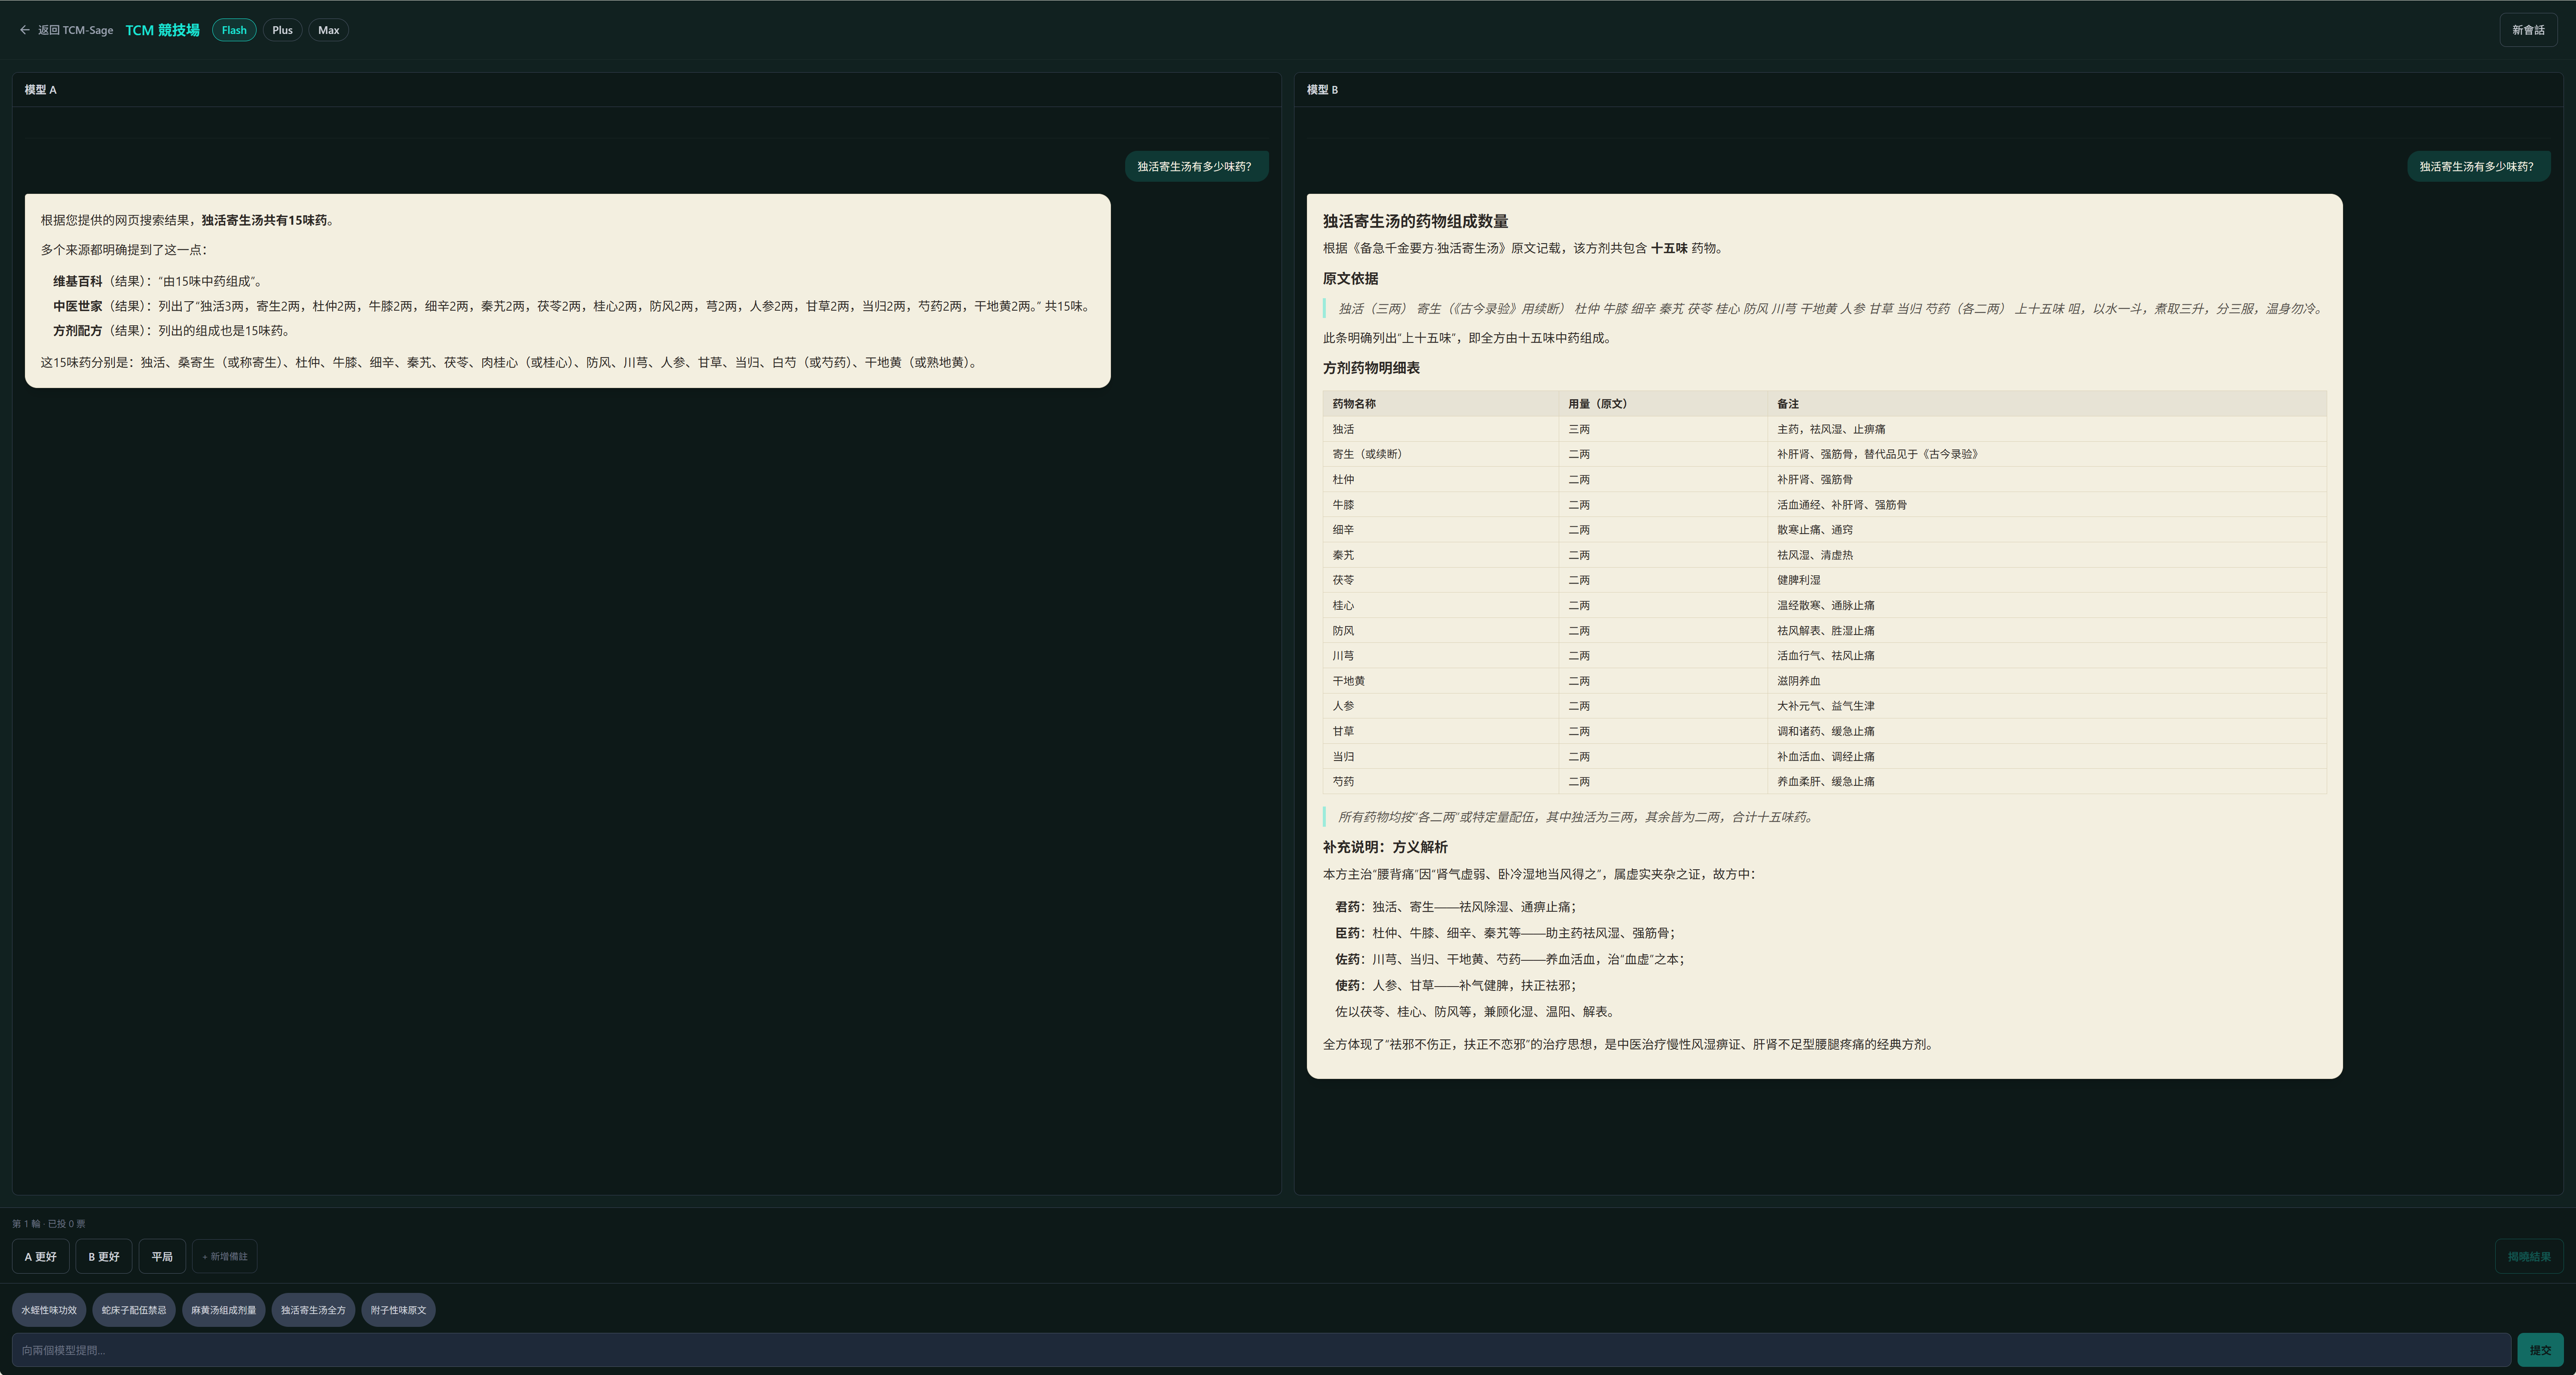
\includegraphics[width=\textwidth]{figures/ui-arena.png}
\caption{The Arena blind A/B evaluation interface with two simultaneous response streams.}
\label{fig:ui_arena}
\end{figure}

\begin{figure}[H]
\centering
\begin{minipage}{0.48\textwidth}
    \centering
    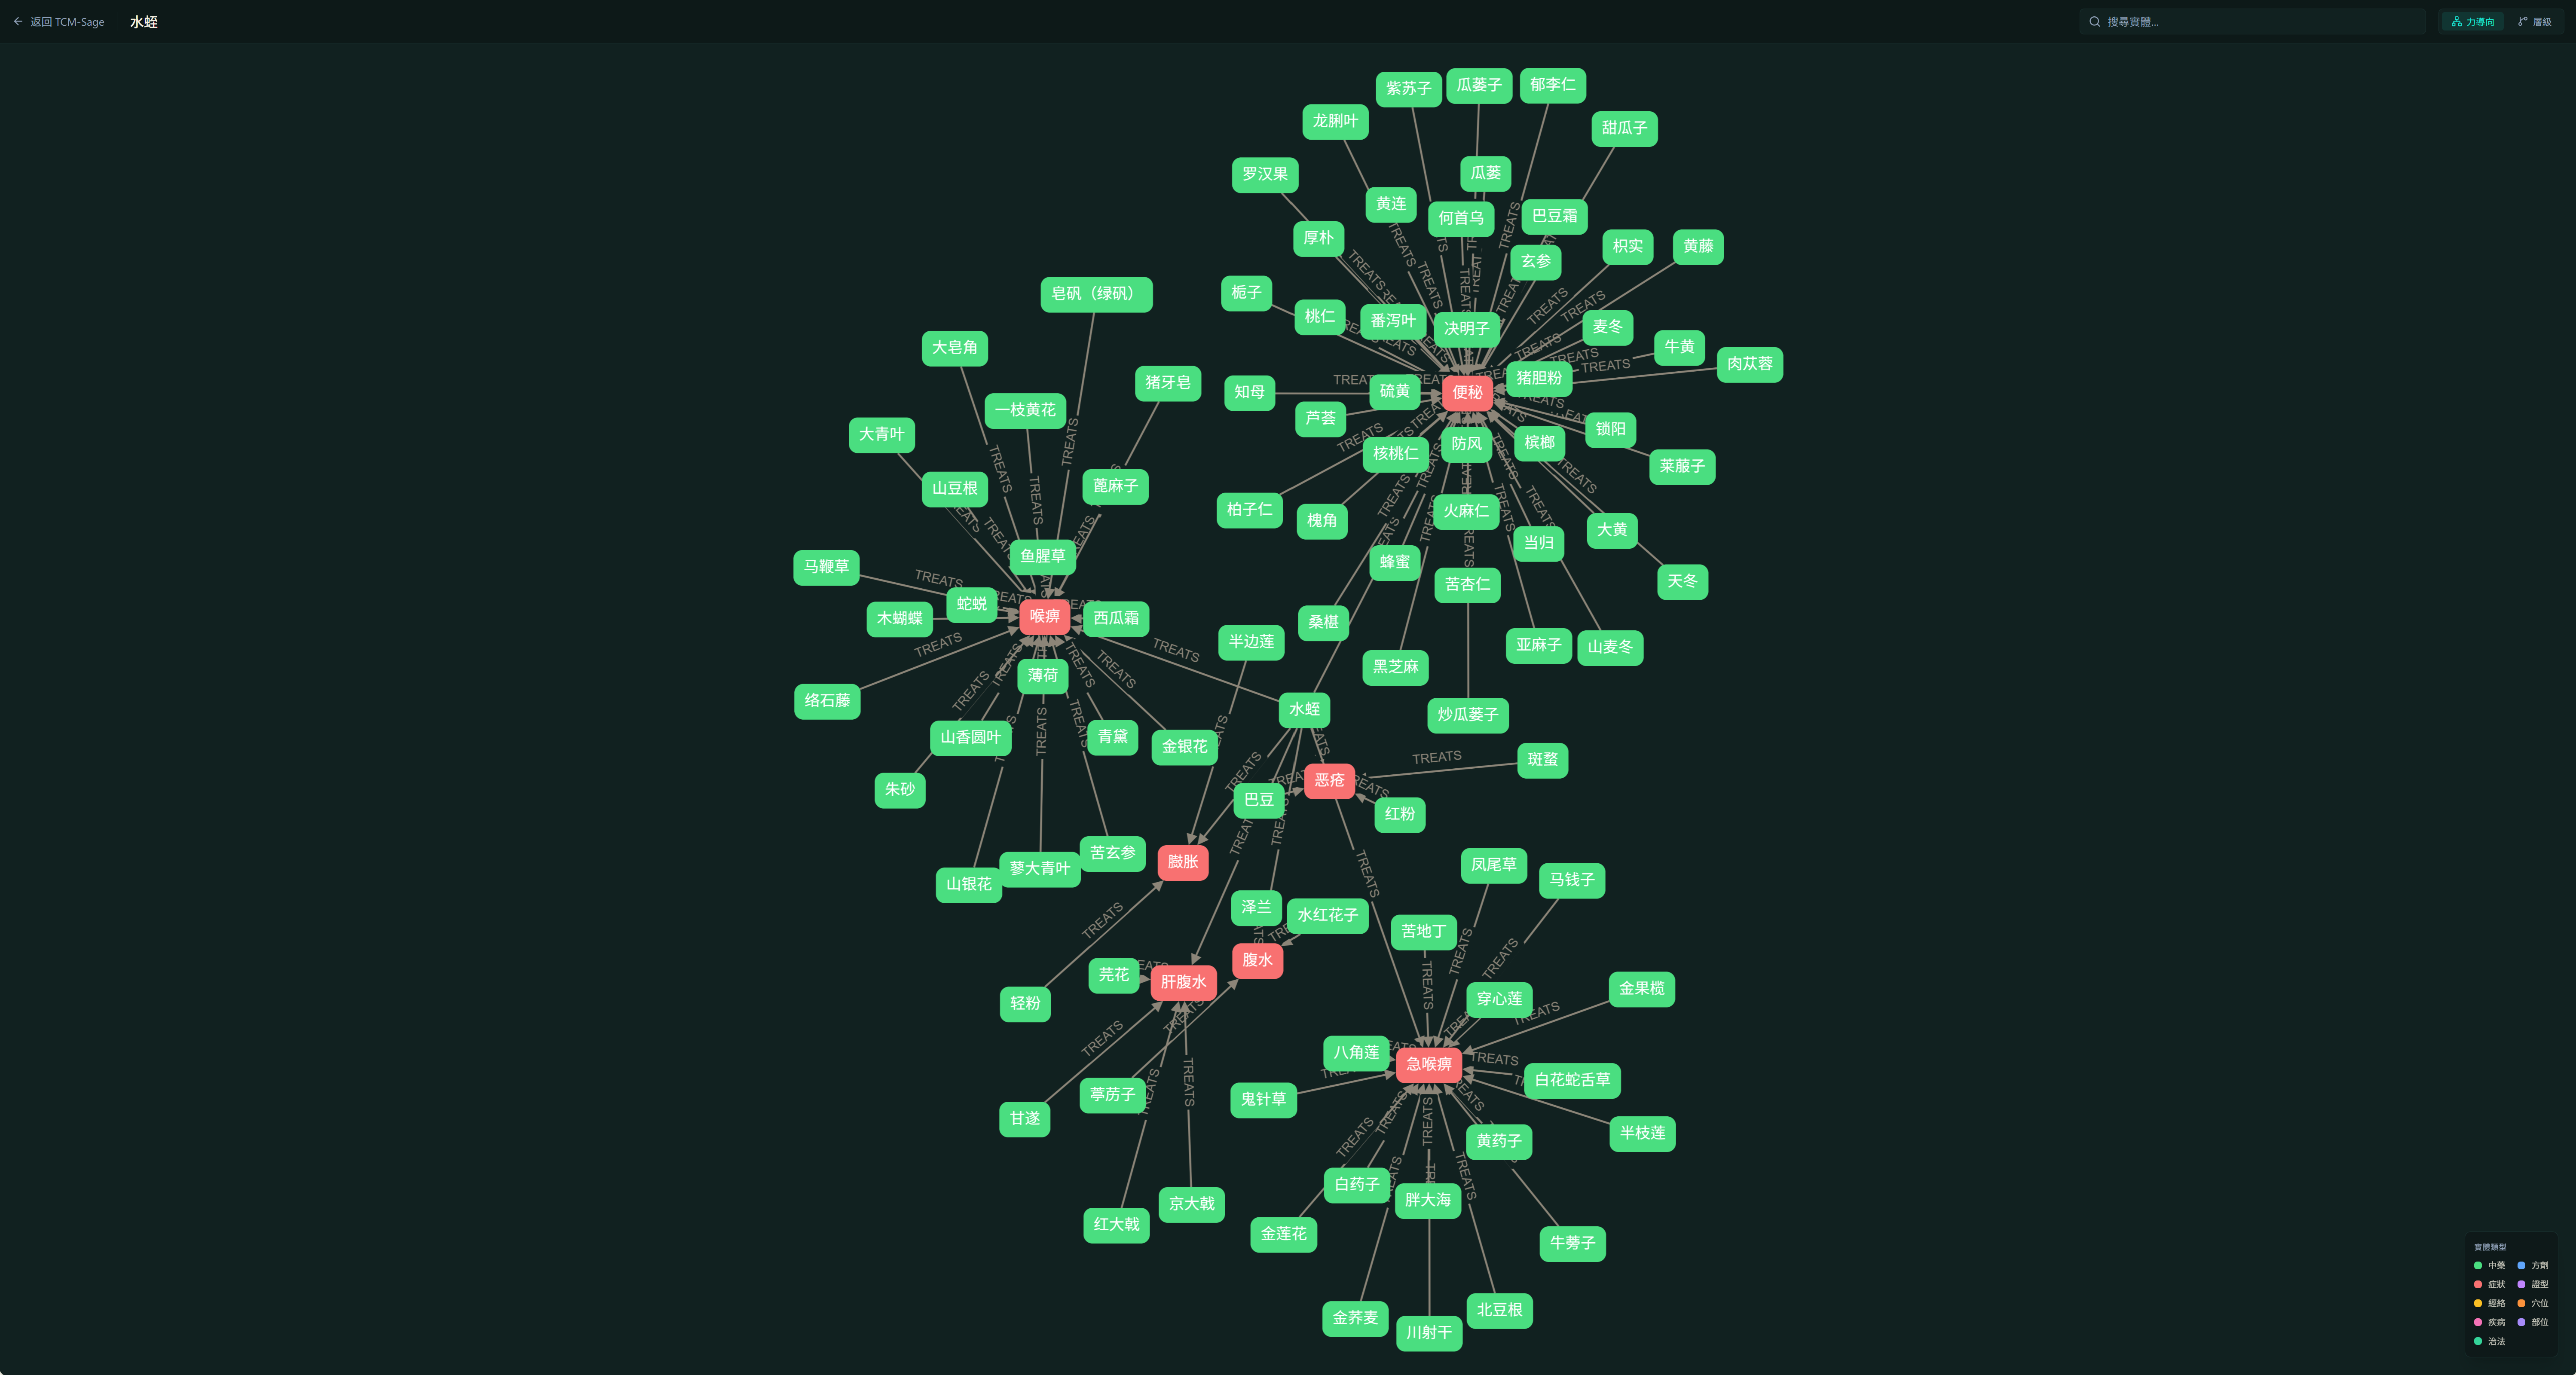
\includegraphics[width=\textwidth]{figures/ui-kg-explorer.png}
    \caption{Full-page Knowledge Graph explorer with entity search and click-to-expand.}
    \label{fig:ui_kg}
\end{minipage}\hfill
\begin{minipage}{0.48\textwidth}
    \centering
    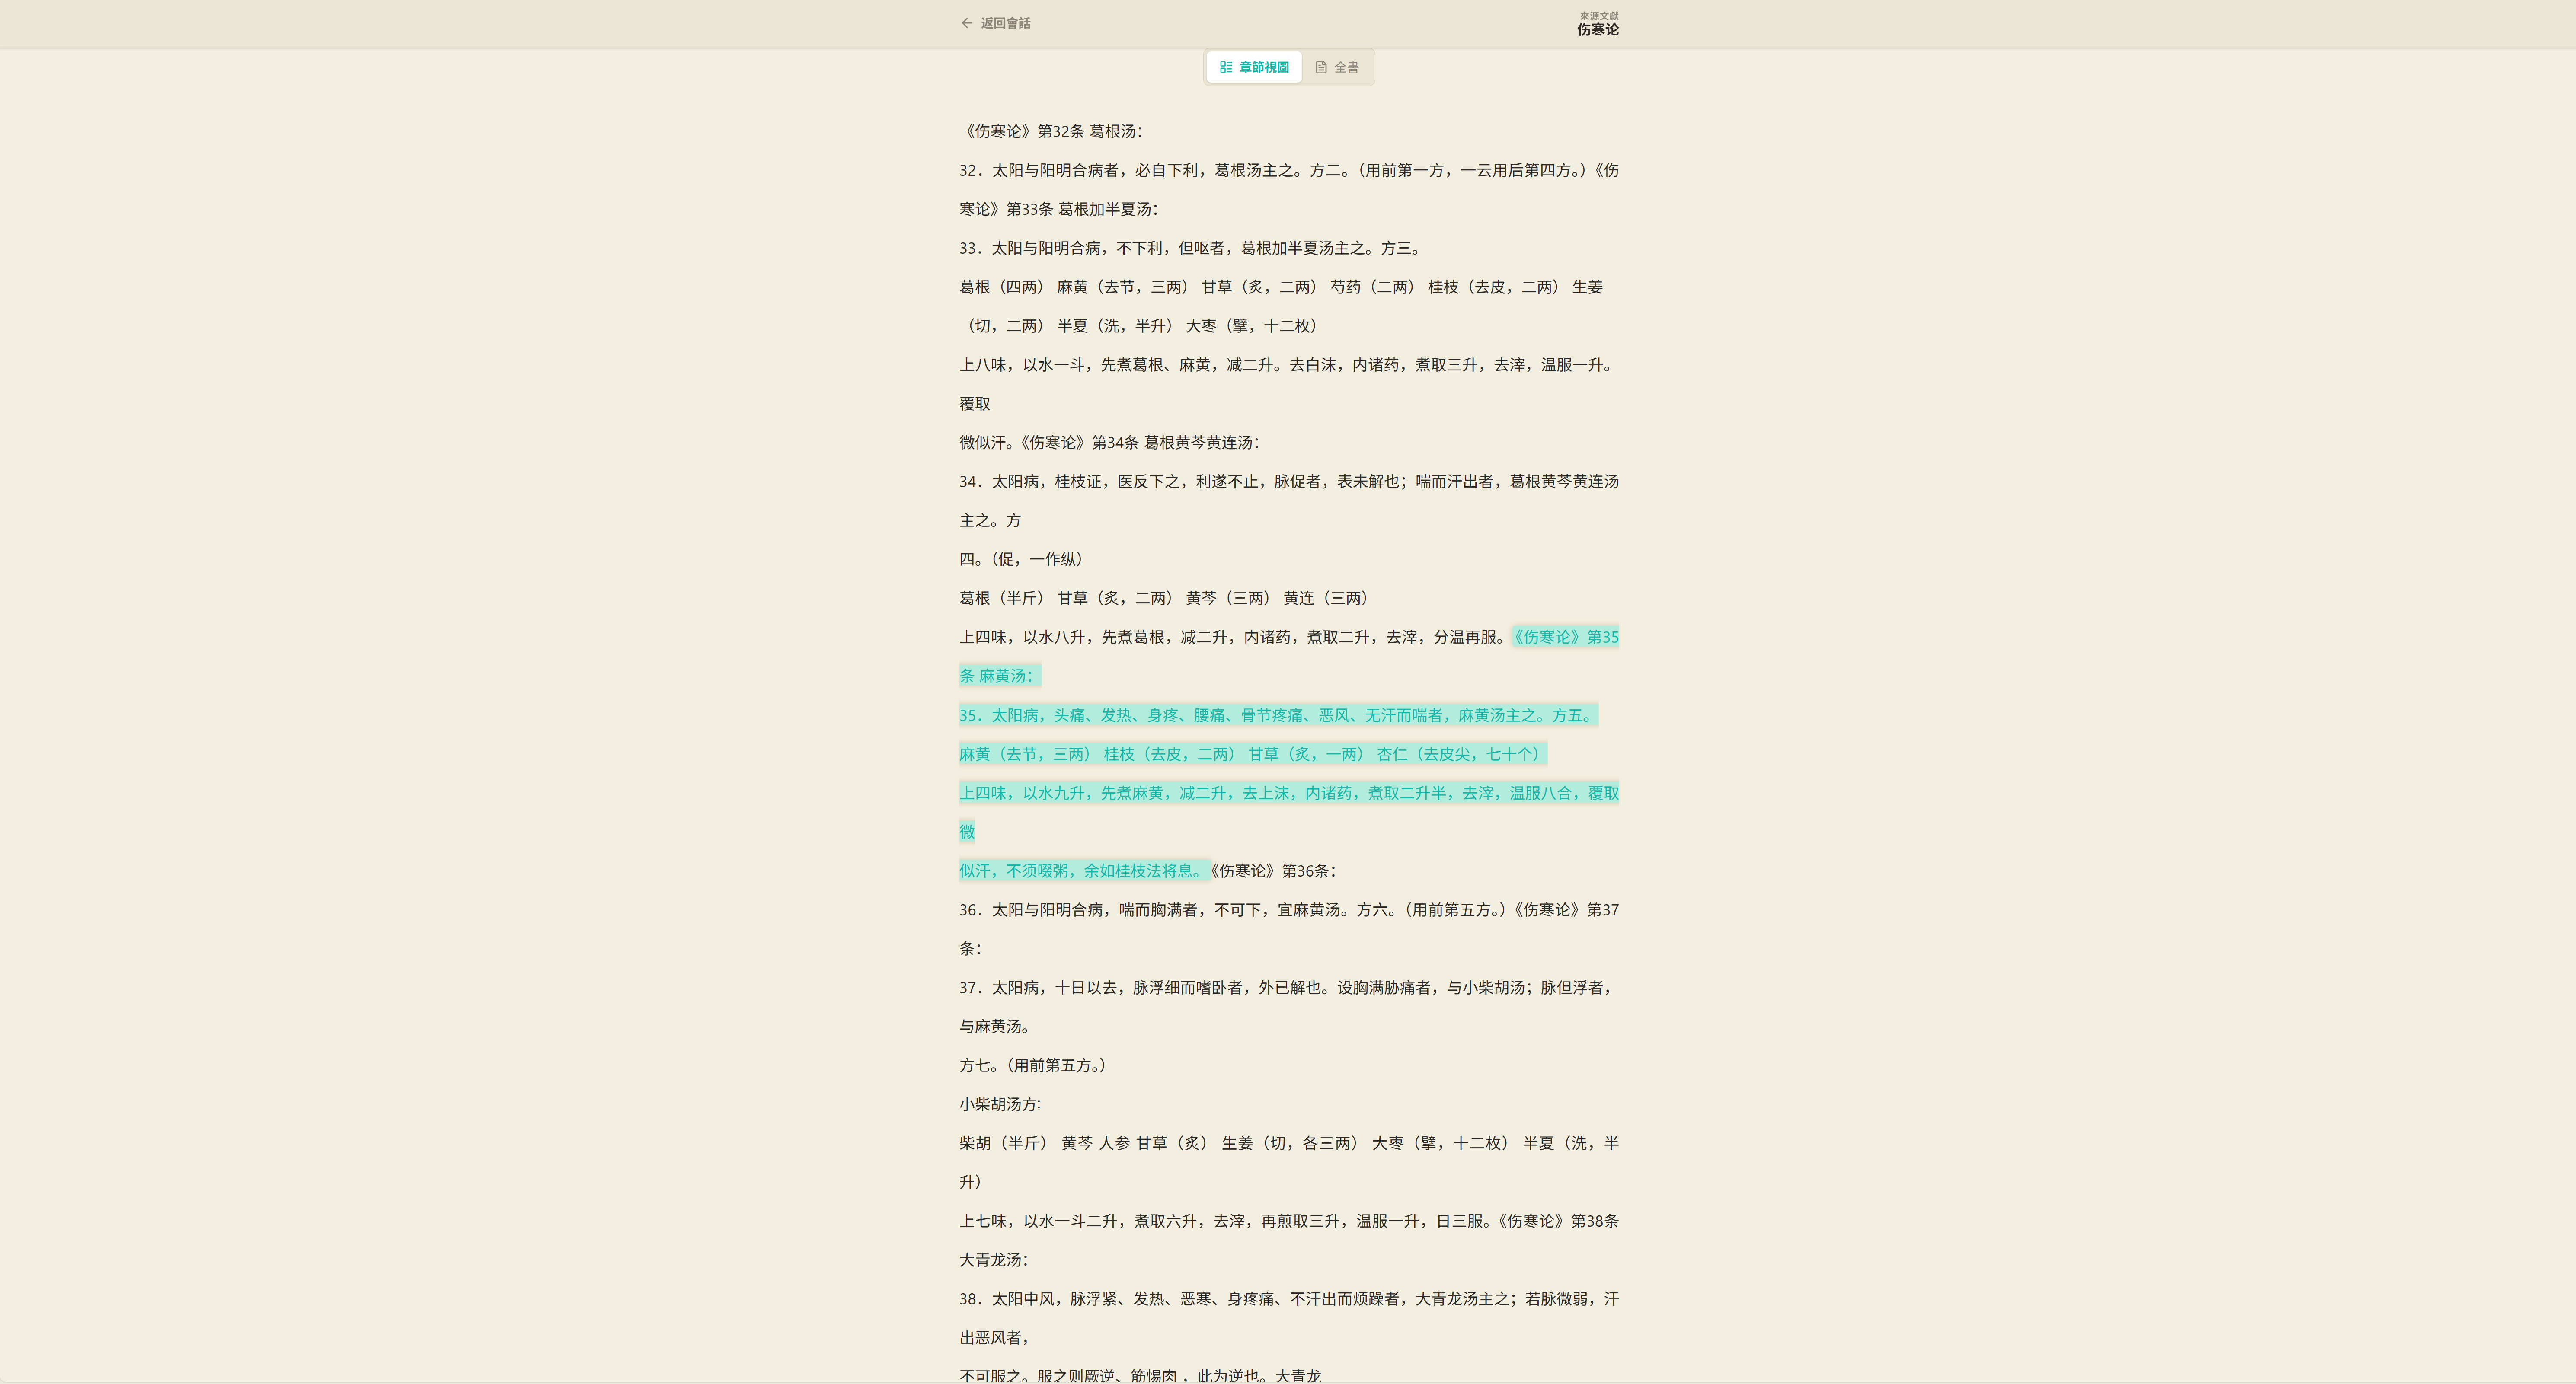
\includegraphics[width=\textwidth]{figures/ui-full-text.png}
    \caption{Full source text viewer showing the original classical passage with metadata.}
    \label{fig:ui_text}
\end{minipage}
\end{figure}

\begin{figure}[H]
\centering
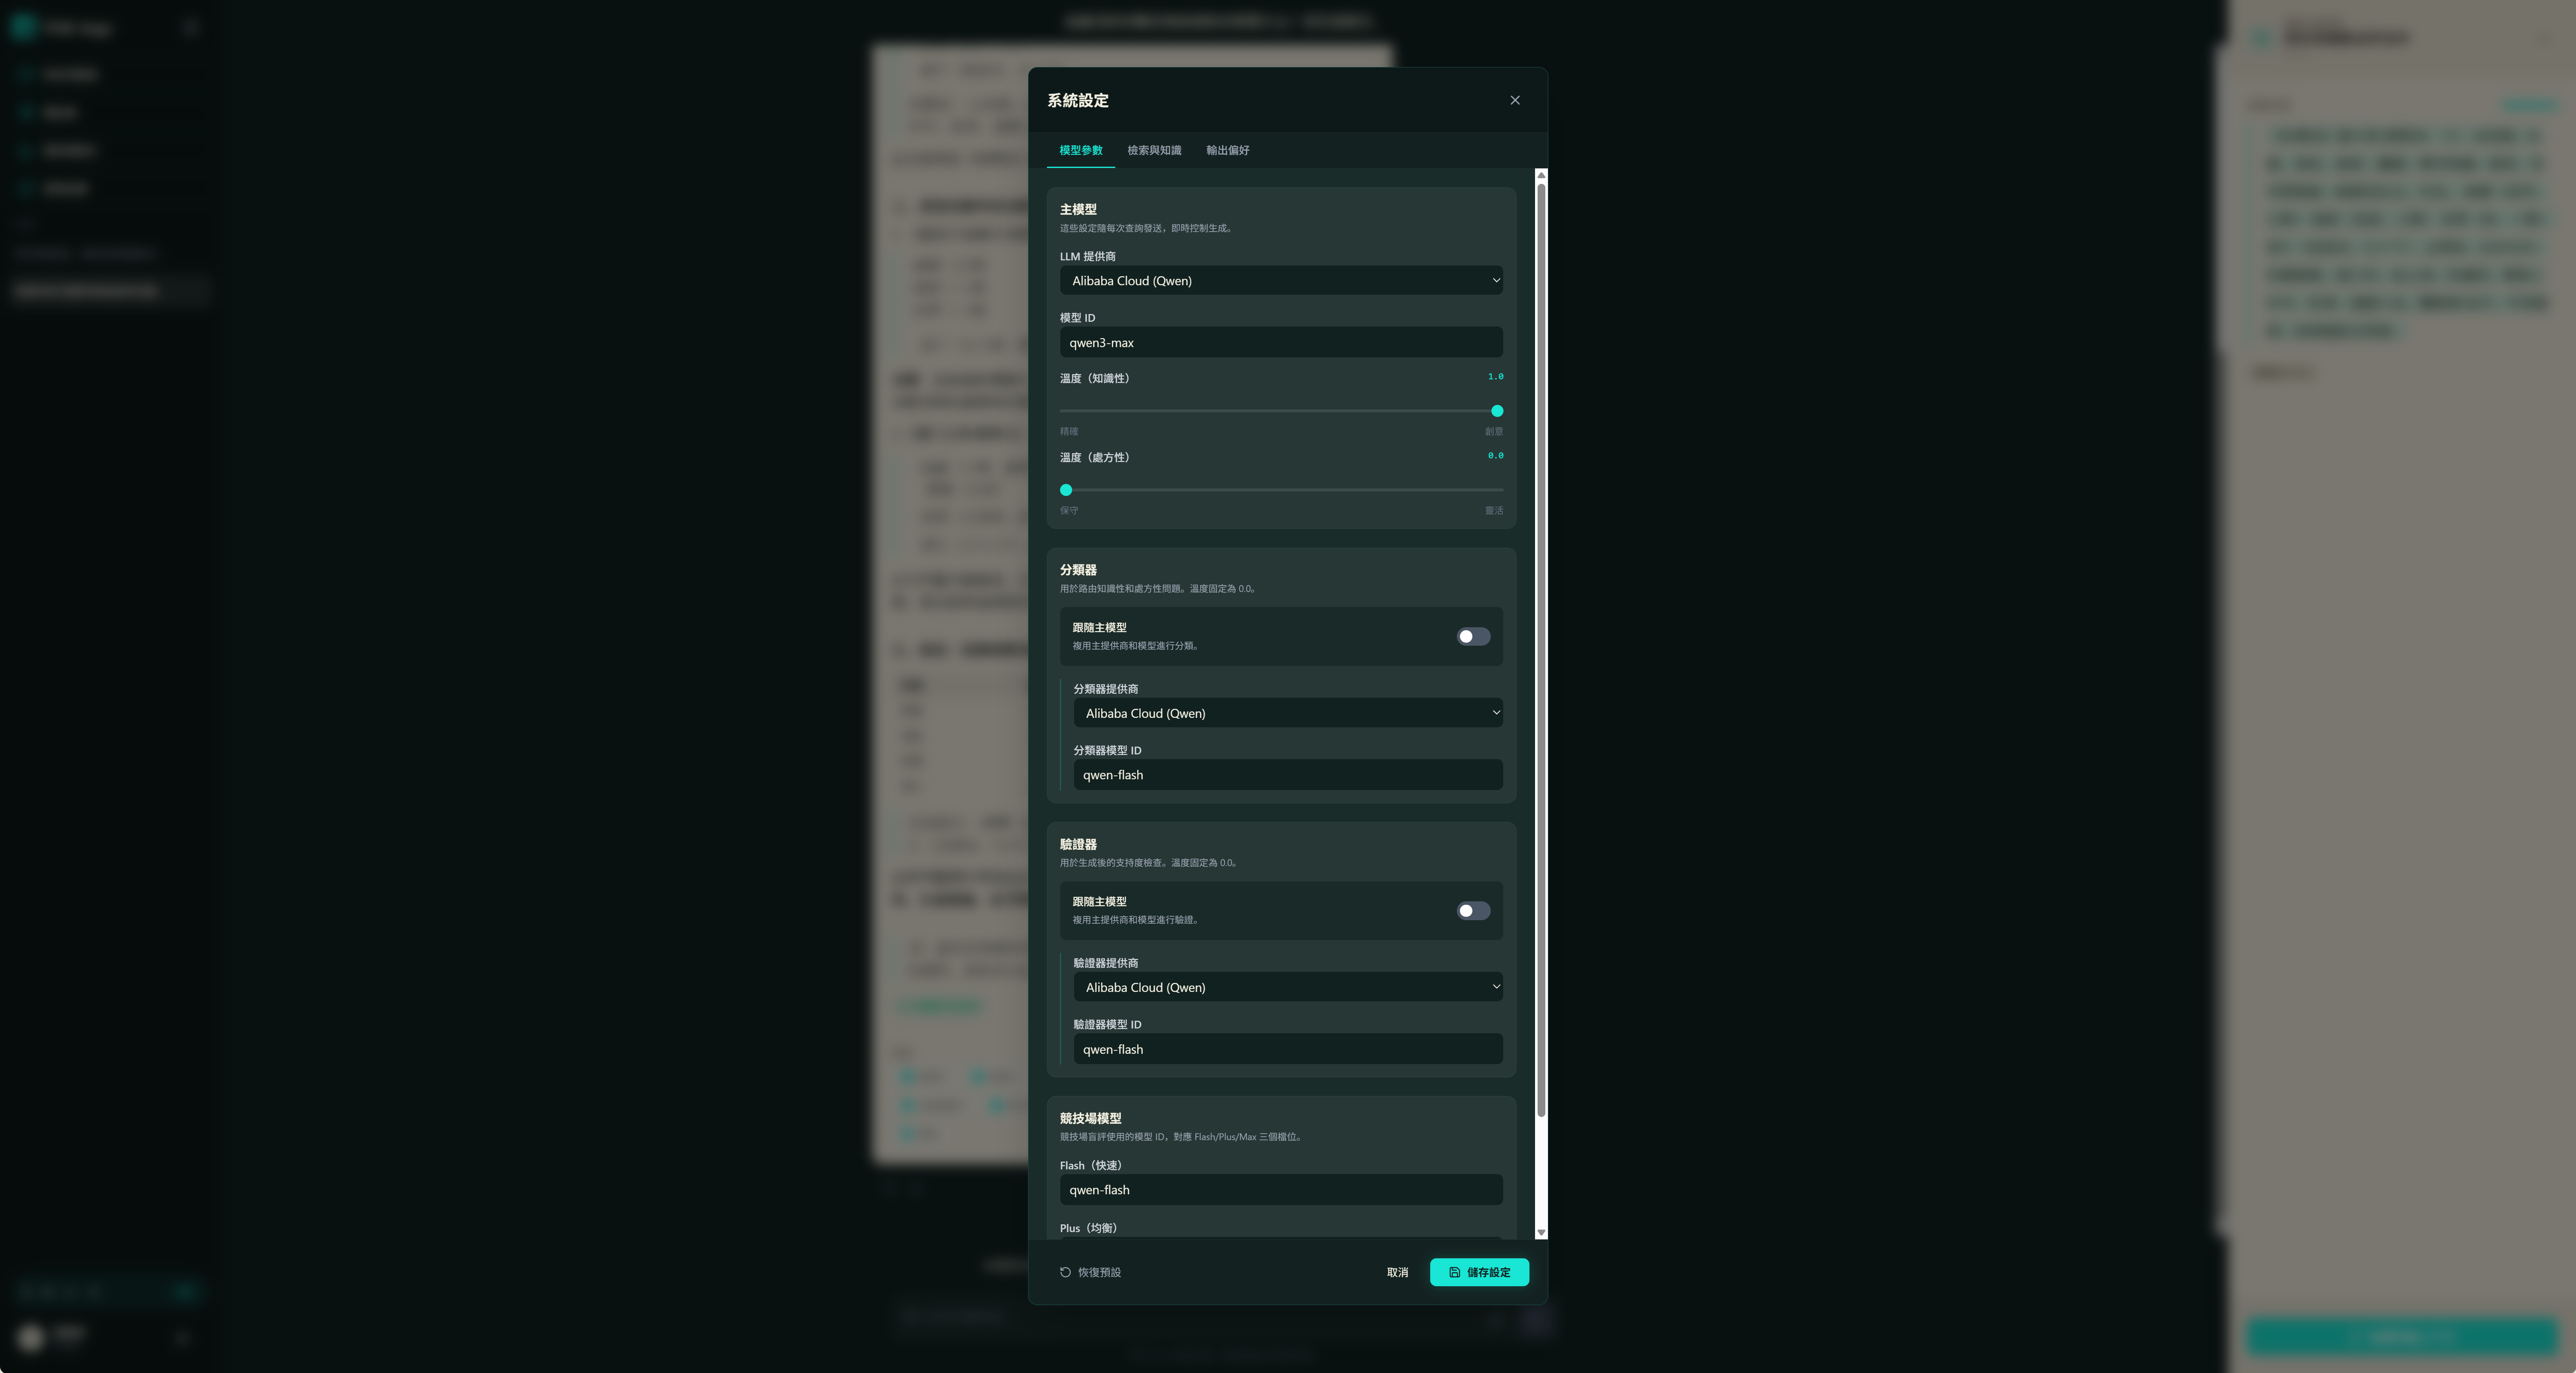
\includegraphics[width=0.5\textwidth]{figures/ui-settings.png}
\caption{The Settings panel allowing configuration of LLM provider, model, and temperature.}
\label{fig:ui_settings}
\end{figure}

\section{Implementation Challenges and Solutions}

\subsection{Retrieval Ranking Bias}
\textbf{Challenge:} Initial testing showed that canonical formula definitions from \textit{Shanghan Lun} were often outranked by lengthy, verbose descriptions in later Ming Dynasty texts (e.g., \textit{Qianjin Fang}), which contained more keyword matches.
\textbf{Solution:} We implemented \textit{Formula-Aware Canonical Retrieval} combined with the \textit{Source Authority Boost}. This ensured that primary sources are always prioritized regardless of their relative brevity compared to later commentaries.

\subsection{RAG Context Engineering}
\textbf{Challenge:} Models like \textit{Qwen-turbo} often ignored formatting rules when the retrieved context exceeded 2,000 characters.
\textbf{Solution:} We adopted "Post-context anchoring," moving the formatting instructions to the very end of the prompt, and utilized \textit{Pattern Priming} by styling the context as Markdown to implicitly guide the model's output structure.

\subsection{Diagnostic Over-Assertion}
\textbf{Challenge:} Early versions of the system would provide definitive diagnoses (e.g., "You have Spleen Deficiency"), which is clinically irresponsible.
\textbf{Solution:} We integrated \textit{Hedging Principles} into the system prompt, requiring the LLM to use uncertain language (e.g., "The symptoms suggest a possibility of...") when evidence is insufficient, and added a mandatory medical disclaimer to all outputs.
